\section{Results}
\label{results}

This section presents quantitative results for the SLM and LLM under RAG, NoRAG, and a hybrid routing strategy. Two \textbf{latency contexts} are used throughout and must not be conflated:
\textbf{(i) Context~A (single-query baseline)}, measured without concurrent load and used for hardware footprint and derived throughput, and
\textbf{(ii) Context~B (concurrent load)}, used for routing, load-testing, and scalability analyses.

Answer quality is evaluated primarily on open benchmarks (label accuracy on MedQA, MMLU-Med, and PubMedQA; $n{=}9{,}090$ per configuration). A supplementary three-query factorial exemplar set ($n{=}3$, Context~B) is used only to demonstrate the token-F1 scoring protocol and is not treated as primary quality evidence.

\subsection{Baseline Comparison (Context~A)}

Figure~\ref{fig:multidimensional} summarizes the SLM--LLM trade-off across six deployment dimensions. Under Context~A, the SLM achieved an inference latency of 2.3\,s, a 4\,GB model footprint, and a derived throughput of 119\,tok/s (273-token mean response length $\div$ 2.3\,s), whereas the LLM required 7.0\,s, 14\,GB, and 60\,tok/s (419 tokens $\div$ 7.0\,s). Because throughput is derived rather than independently benchmarked, it should be interpreted with care: under Context~B concurrent load (22.18\,s for the SLM and 49.55\,s for the LLM), effective per-request throughput is substantially lower.

\begin{figure}[t]
\centering
\includegraphics[width=\columnwidth]{fig_multidimensional_comparison.pdf}
\caption{Multidimensional comparison of SLM and LLM across six performance 
dimensions under Context~A baseline conditions.}
\label{fig:multidimensional}
\end{figure}

\subsection{Query Set and Mapping to Tables}

Table~\ref{tab:query-mapping} lists the curated evaluation queries and their corresponding analyses. Queries Q1--Q3 form the core 2$\times$2 factorial exemplar set used for curated-set token-F1 comparisons, while Q4--Q12 support the routing and load-testing experiments.

\begin{table}[t]
\centering
\caption{Query set and mapping to results (Q1--Q3 exemplars; Q4--Q12 extended set).}
\label{tab:query-mapping}
\footnotesize
\setlength{\tabcolsep}{3pt}
\renewcommand{\arraystretch}{1.1}

\begin{tabular}{l|p{0.46\columnwidth}|p{0.36\columnwidth}}
\hline
\textbf{ID} & \textbf{Query (abbreviated)} & \textbf{Used in} \\
\hline

Q1--Q3 & Diabetes / AI diagnosis / hypertension (factorial exemplars) & Fig.~\ref{fig:rag-scenario-responses}; Sec.~\ref{sec:routing-discussion} \\

Q4--Q12 & ACS/NSCLC/stroke/COVID-19/insulin/sepsis/HFpEF/CAR-T/anticoagulation & Routing, load test, scalability \\

\hline
\end{tabular}

\end{table}

\subsection{Corpus Statistics and Index Properties}
\label{results:corpus}

The indexed corpus comprised 115 sources yielding 556 semantic chunks (Section~\ref{phase1}). The FAISS index was approximately 100\,MB, and retrieval latency ranged from 50--100\,ms per query.

\subsection{Retrieval Performance}
\label{results:retrieval}

Retrieval quality was assessed using the hybrid dense--sparse index employed at inference (FAISS dense search with lexical BM25 re-ranking). For benchmark items with a known gold source chunk, \textbf{Recall@$k$} denotes the fraction of gold-relevant chunks found among the top-$k$ retrieved results, and \textbf{MRR} denotes the mean reciprocal rank of the first gold hit. Table~\ref{tab:retrieval-performance} reports these metrics on the \textbf{gold-label evaluable subset} $n{=}3{,}300$ per RAG configuration rows. For reference, pooling across 34 merged evaluation runs over all retrieval-attempted rows yields Recall@3 $=$ 0.919 and MRR $=$ 0.997; these supplementary figures are not used as the headline retrieval result.

\begin{table*}[htbp]
\centering
\caption{Retrieval performance on the shared hybrid index ($n{=}3{,}300$ gold-evaluable rows per RAG configuration). Both SLM+RAG and LLM+RAG use the identical FAISS+BM25 index.}
\label{tab:retrieval-performance}
\footnotesize
\setlength{\tabcolsep}{4pt}
\renewcommand{\arraystretch}{1.1}
\begin{tabular}{lccccc}
\toprule
\textbf{Configuration} &
\textbf{Recall@1} &
\textbf{Recall@3} &
\textbf{Recall@5} &
\textbf{Recall@10} &
\textbf{MRR} \\
\midrule
\textbf{RAG (both models)} & 0.667 & 0.891 & 0.914 & 0.936 & 0.967 \\

\bottomrule
\end{tabular}
\end{table*}

Strong gold-subset retrieval performance, however, did not translate uniformly into downstream accuracy gains on the open benchmarks (Table~\ref{tab:answer-quality}).

\subsection{Retrieval-Augmented Generation Effectiveness}
\label{results:rag}

RAG increased the amount of evidence-conditioned text generated by both models. Response length is reported only as a proxy for content quantity and should not be interpreted as a measure of correctness. Figure~\ref{fig:rag-scenario-responses} shows per-scenario token counts for Q1--Q3; answer quality was evaluated separately via benchmark accuracy (Table~\ref{tab:answer-quality}) and curated-set token-F1 (Section~\ref{sec:routing-discussion}).

With RAG enabled, mean response length increased from 273 to 454 tokens (+66.3\%) for the SLM and from 419 to 484 tokens (+15.5\%) for the LLM (Figure~\ref{fig:rag-scenario-responses}). Open-benchmark accuracy is reported in Table~\ref{tab:answer-quality}; curated token-F1 on three exemplar queries ($n{=}3$, Context~B) is reported in Section~\ref{sec:routing-discussion} as an illustrative methodology demonstration only and should not be conflated with open-benchmark macro-F1 or treated as a main quality conclusion.

\begin{figure}[t]
\centering
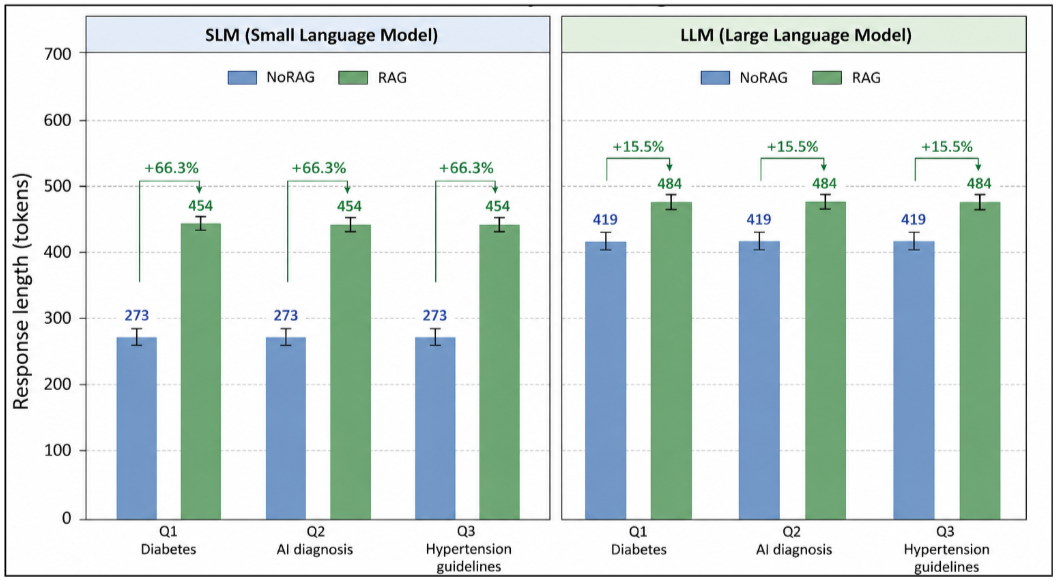
\includegraphics[width=\columnwidth]{fig_rag_scenario_responses.png}
\caption{Effect of RAG on response length (tokens) across three clinical 
scenarios for SLM and LLM.}
\label{fig:rag-scenario-responses}
\end{figure}

\subsection{Routing, Latency, and Efficiency}
\label{sec:routing-discussion}

\subsubsection{Intelligent query routing}

The routing component is a \textbf{rule-based heuristic classifier} (not a learned model) that combines four lexical features---average word length (weight 0.5141), query complexity (0.3824), word count (0.0852), and entity count (0.0183)---implemented in \texttt{eval\_routing.py}. Implementation consistency on the 240-query definition set is reported in Appendix~\ref{app:routing-consistency} and is not interpreted as held-out routing accuracy. The \textbf{primary routing evidence} is behavioral: across the 12-query extended set (Q1--Q12), 68\% of queries were routed to the SLM, 24\% to the LLM, and the remaining $\approx$8\% fell into an intermediate region handled by a deterministic fallback that defaults to the LLM.

\begin{figure}[t]
\centering
\includegraphics[width=\columnwidth]{fig_feature_importance.pdf}
\caption{Feature importance for query routing; average word length and query complexity dominate.}
\label{fig:feature-importance}
\end{figure}

\begin{table*}[htbp]
\centering
\caption{Answer quality (mean accuracy) and faithfulness (0--100, RAG rows only) by configuration ($n{=}9{,}090$ per row).}
\label{tab:answer-quality}
\footnotesize
\setlength{\tabcolsep}{4pt}
\renewcommand{\arraystretch}{1.05}
\begin{tabular}{l|c|c|c|c|c}
\toprule
\textbf{Configuration} &
\textbf{MedQA} &
\textbf{MMLU-Med} &
\textbf{PubMedQA} &
\textbf{ROUGE-L} &
\textbf{Faithfulness (\%)} \\
\midrule
SLM (No RAG) & 0.404 & 0.510 & 0.622 & 0.556 & N/A \\
SLM + RAG    & 0.403 & 0.518 & 0.596 & 0.562 & 47.2 \\
LLM (No RAG) & 0.365 & 0.421 & 0.523 & 0.328 & N/A \\
LLM + RAG    & 0.348 & 0.499 & 0.494 & 0.142 & 47.8 \\
\bottomrule
\end{tabular}
\end{table*}

\textbf{ROUGE-L drop under LLM+RAG (PubMedQA).}
The opposing ROUGE-L and token-F1 trends observed for LLM+RAG on PubMedQA warrant explanation. PubMedQA reference answers are short classification labels (``yes,'' ``no,'' or ``maybe''), which makes ROUGE-L highly sensitive to response verbosity: because RAG increases the LLM's mean response length toward 484 tokens, ROUGE-L falls (0.328$\rightarrow$0.142) relative to these terse references, even as token-F1 computed against the retrieved-chunk vocabulary rises (0.049$\rightarrow$0.172). SLM ROUGE-L, by contrast, remains stable (0.556$\rightarrow$0.562). \textbf{Label accuracy} in Table~\ref{tab:answer-quality} remains the primary PubMedQA metric; ROUGE-L is reported for completeness only.

\subsubsection{Benchmark error analysis}
\label{results:error-analysis}

Table~\ref{tab:answer-quality} shows that RAG did not uniformly improve label accuracy. Three factors help explain these mixed outcomes.

\textbf{Corpus--benchmark mismatch (MedQA).}
MedQA items often require reasoning over USMLE-style clinical vignettes whose topical coverage is broader than our 115-document corpus (112 PubMed articles and three guidelines). When retrieved segments are only weakly related to the vignette, RAG can inject off-topic context that competes with parametric knowledge. This plausibly explains the small MedQA decreases under RAG (SLM: 0.404$\rightarrow$0.403; LLM: 0.365$\rightarrow$0.348) despite strong gold-subset retrieval metrics (Recall@3 $=0.891$).

\textbf{Response-format mismatch (PubMedQA).}
PubMedQA is scored by short yes/no/maybe labels, whereas RAG prompts encourage longer evidence-grounded explanations. The LLM+RAG configuration therefore shows lower PubMedQA label accuracy (0.523$\rightarrow$0.494) alongside increased verbosity, consistent with format mismatch rather than uniformly worse medical content.

\textbf{Model--task interaction (LLM vs.\ SLM).}
On the open benchmarks, Gemma-2-2B-it (SLM) outperformed Llama-2-7B-chat (LLM) on MedQA and PubMedQA in both NoRAG and RAG settings. This may reflect instruction-tuning differences, decoding behavior, or benchmark-format sensitivity rather than a general claim that smaller models are clinically superior. The primary conclusion supported by $n{=}9{,}090$ predictions per configuration is that RAG effects are \emph{task dependent}, not uniformly beneficial.

\textbf{Partial faithfulness ($\approx$47--48\%).}
Automated faithfulness scores near 50\% indicate that roughly half of judged answer content received only partial or indirect support from retrieved passages under the Qwen2.5-7B-Instruct rubric (40--55 partial-support band). This is consistent with retrieval noise, multi-claim answers in which only some sentences are grounded, and strict judge criteria. It motivates corpus expansion, reranking refinement, and quantitative Phase~4 claim-verifier blocking rates in future work.

\begin{figure}[t]
\centering
\includegraphics[width=\columnwidth]{fig_routing_decisions.pdf}
\caption{Routing confidence vs.\ latency per query on the Q1--Q12 workload set.}
\label{fig:routing-decisions}
\end{figure}

\subsubsection{Static and routing comparison under load}

Under Context~B concurrent load on Q1--Q12, the SLM-only, LLM-only, and hybrid-routing strategies occupy distinct positions on the latency frontier. A supplementary three-query token-F1 exemplar ($n{=}3$) is reported only in the limitations (Section~\ref{discussion}) to demonstrate the scoring protocol and is not used as primary quality evidence.

\subsection{Clinical Answer Quality (LLM-as-Judge)}
\label{results:llm-judge}

Model-based clinical scoring complements the overlap-based metrics. Qwen/Qwen2.5-7B-Instruct rated each response on a 0--5 rubric for \emph{correctness}, \emph{completeness}, and \emph{clinical relevance}. Figure~\ref{fig:llm-judge-scores} reports mean scores on the judged subset ($n{=}8{,}950$ for SLM+RAG and $n{=}8{,}965$ for all other configurations). Coverage was 35,845 of 36,360 predictions (98.6\%), with 515 rows left unjudged (140 for SLM\_RAG and 125 for each remaining configuration).

\begin{figure}[t]
\centering
\includegraphics[width=\columnwidth]{fig_llm_judge_scores.pdf}
\caption{LLM-as-judge clinical scores (Qwen2.5-7B-Instruct; 0--5 scale). RAG vs.\ NoRAG differences are negligible in effect size.}
\label{fig:llm-judge-scores}
\end{figure}

RAG-versus-NoRAG judge-score differences were small ($|\Delta| \leq 0.13$; Cohen's $d < 0.15$). These scores reflect within-run rankings rather than evidence of clinical approval.

\subsection{Scalability and System Stability}

Latency increased non-linearly with user load: scaling from 5 to 10 concurrent users increased latency by approximately 2.24$\times$. All configurations maintained stable token generation without truncation. Peak GPU memory under concurrent load is reported in Table~\ref{tab:eie-infrastructure}.


\subsection{EIE Framework Assessment}
\label{results:eie}

Deployability was assessed using the \textbf{EIE (Energy--Infrastructure--Economy) Framework} defined in Section~\ref{methodology:eie} (Figure~\ref{fig:eie-framework}). GPU energy was measured via NVML telemetry across 10 trials $\times$ 20 clinical queries per strategy~\cite{patterson2021carbon,strubell2019energy}. \textbf{Scope:} all Pillar~E measurements are GPU-scoped only and exclude data-center overhead. Carbon emissions were derived from measured kWh using $\gamma_{\mathrm{grid}} = 0.385$\,kg CO\textsubscript{2}e/kWh~\cite{epa2023egrid}; \textbf{kWh/query} remains the primary, grid-independent metric. Pillar observables are reported separately from clinical accuracy and faithfulness (Table~\ref{tab:answer-quality}).

\subsubsection{Pillar E: Energy and carbon emissions}

Table~\ref{tab:energy-carbon} reports per-query GPU energy (mean$\,\pm$\,std) and derived CO\textsubscript{2}e for all five strategies. Figure~\ref{fig:eie-energy-carbon} visualizes the same Pillar~E observables: per-query energy intensity (bars) and derived CO\textsubscript{2}e per million queries (line). RAG added negligible mean energy ($<$2\%) relative to NoRAG within each model class, and pairwise kWh ratios are invariant to grid carbon intensity~\cite{ren2024reconciling}.

\begin{table}[htbp]
\centering
\caption{Pillar~E: per-query GPU energy and derived carbon (NVML; $\gamma_{\mathrm{grid}} = 0.385$\,kg/kWh; GPU-scoped, excludes data-center overhead).$^{*}$}
\label{tab:energy-carbon}
\footnotesize
\setlength{\tabcolsep}{4pt}
\renewcommand{\arraystretch}{1.12}
\begin{tabular}{l|c|c}
\toprule
\textbf{Strategy} & \textbf{kWh/query} & \textbf{CO\textsubscript{2}e/M (kg)} \\
\midrule
SLM\_NoRAG      & 0.000052 $\pm$ 0.000011 & 19.83 \\
SLM\_RAG        & 0.000052 $\pm$ 0.000013 & 19.82 \\
LLM\_NoRAG      & 0.000111 $\pm$ 0.000024 & 42.35 \\
LLM\_RAG        & 0.000112 $\pm$ 0.000023 & 42.47 \\
Routing\_Hybrid & 0.000101 $\pm$ 0.000021 & 38.19 \\
\bottomrule
\end{tabular}

\vspace{2pt}
\noindent\footnotesize $^{*}$CO\textsubscript{2}e/M from full-precision kWh means; displayed kWh rounded ($\leq$1.8\% mismatch). GPU scope only.
\end{table}

\begin{figure}[htbp]
\centering
\includegraphics[width=\columnwidth]{fig_eie_energy_carbon.pdf}
\caption{Pillar~E: per-query energy intensity (kWh/query) and derived CO\textsubscript{2}e per million queries across deployment strategies. SLM\_RAG consumed approximately 2.15$\times$ less energy per query than LLM\_RAG.}
\label{fig:eie-energy-carbon}
\end{figure}

\subsubsection{Pillar I: Infrastructure}

Table~\ref{tab:eie-infrastructure} summarizes the Pillar~I observables.

\begin{table}[htbp]
\centering
\caption{Pillar~I: infrastructure observables (SLM+RAG vs.\ LLM+RAG).}
\label{tab:eie-infrastructure}
\footnotesize
\setlength{\tabcolsep}{4pt}
\renewcommand{\arraystretch}{1.1}
\begin{tabular}{l|c|c|c}
\toprule
\textbf{Metric} & \textbf{SLM+RAG} & \textbf{LLM+RAG} & \textbf{Ratio} \\
\midrule
VRAM footprint (GB) & 4 & 14 & 3.50$\times$ \\
Latency Context~A (s) & 2.3 & 7.0 & 3.04$\times$ \\
Latency Context~B (s) & 22.18 & 49.55 & 2.23$\times$ \\
Throughput (tok/s) & 119 & 60 & 1.98$\times$ \\
Peak GPU load (GB) & \multicolumn{2}{c|}{14.28--14.37} & N/A \\
\bottomrule
\end{tabular}

\vspace{2pt}
\noindent\footnotesize $^{\ddagger}$Derived from Context~A only.
\end{table}

\subsubsection{Pillar Ec: Economy (electricity and hardware cost)}

Electricity operating expense was computed from measured kWh using a reference U.S.\ tariff of \$0.12/kWh, and hardware amortization assumes reference GPU capex tiers depreciated over three years. Table~\ref{tab:eie-economy} summarizes the annual electricity and amortized hardware costs by strategy.

\begin{table}[htbp]
\centering
\caption{Pillar~Ec: annual electricity and amortized hardware cost (USD reference tariffs).}
\label{tab:eie-economy}
\footnotesize
\setlength{\tabcolsep}{3pt}
\renewcommand{\arraystretch}{1.1}
\begin{tabular}{l|c|c|c}
\toprule
\textbf{Strategy} & \textbf{Elec./yr} & \textbf{GPU amort./yr} & \textbf{Combined/yr} \\
\midrule
SLM\_RAG & \$2{,}278 & \$117 & \$2{,}395 \\
LLM\_RAG & \$4{,}901 & \$400 & \$5{,}301 \\
Routing\_Hybrid & \$4{,}422 & \$400 & \$4{,}822 \\
\bottomrule
\end{tabular}

\vspace{2pt}
\noindent\footnotesize Elec./yr = measured kWh $\times$ \$0.12; hardware amort.\ = reference capex $\div$ 3 yr.
\end{table}